%\def\year{2022}\relax
%File: formatting-instructions-latex-2022.tex
%release 2022.1
%\documentclass[letterpaper]{article} % DO NOT CHANGE THIS
%\usepackage{aaai22}  % DO NOT CHANGE THIS
%\usepackage{times}  % DO NOT CHANGE THIS
%\usepackage{helvet}  % DO NOT CHANGE THIS
%\usepackage{courier}  % DO NOT CHANGE THIS
%\usepackage[hyphens]{url}  % DO NOT CHANGE THIS
%\usepackage{graphicx} % DO NOT CHANGE THIS
%\urlstyle{rm} % DO NOT CHANGE THIS
%\def\UrlFont{\rm}  % DO NOT CHANGE THIS
%\usepackage{natbib}  % DO NOT CHANGE THIS AND DO NOT ADD ANY OPTIONS TO IT
%\usepackage{caption} % DO NOT CHANGE THIS AND DO NOT ADD ANY OPTIONS TO IT
%\DeclareCaptionStyle{ruled}{labelfont=normalfont,labelsep=colon,strut=off} % DO NOT CHANGE THIS
%\frenchspacing  % DO NOT CHANGE THIS
%\setlength{\pdfpagewidth}{8.5in}  % DO NOT CHANGE THIS
%\setlength{\pdfpageheight}{11in}  % DO NOT CHANGE THIS
%
% These are recommended to typeset algorithms but not required. See the subsubsection on algorithms. Remove them if you don't have algorithms in your paper.
%\usepackage{algorithm}
%\usepackage{algorithmic}

%
% These are are recommended to typeset listings but not required. See the subsubsection on listing. Remove this block if you don't have listings in your paper.
%\usepackage{newfloat}
%\usepackage{listings}
%\lstset{%
%	basicstyle={\footnotesize\ttfamily},% footnotesize acceptable for monospace
%	numbers=left,numberstyle=\footnotesize,xleftmargin=2em,% show line numbers, remove this entire line if you don't want the numbers.
%	aboveskip=0pt,belowskip=0pt,%
%	showstringspaces=false,tabsize=2,breaklines=true}
%\floatstyle{ruled}
%\newfloat{listing}{tb}{lst}{}
%\floatname{listing}{Listing}
%ADD
%\usepackage{hhline}
%\usepackage{booktabs}
%\usepackage{multirow}
%\usepackage{subfigure}
%\usepackage{amsmath}
%\newcommand{\figref}[1]{Figure \ref{#1}}
%\newcommand{\eqnref}[1]{Eq. \ref{#1}}
%\newcommand{\tabref}[1]{Table \ref{#1}}
%\newcommand{\secref}[1]{Section \ref{#1}}
%\newcommand{\algoref}[1]{Algorithm \ref{#1}}
%\usepackage{makecell}
%\usepackage{color}
%\newcommand{\KZ}[1]{\textcolor{red}{Kenny: #1}}
%\newcommand{\YZ}[1]{\textcolor{green}{Yizhu: #1}}
%\newcommand{\JQ}[1]{\textcolor{green}{JQ: #1}}
%
%\nocopyright
%
% PDF Info Is REQUIRED.
% For /Title, write your title in Mixed Case.
% Don't use accents or commands. Retain the parentheses.
% For /Author, add all authors within the parentheses,
% separated by commas. No accents, special characters
% or commands are allowed.
% Keep the /TemplateVersion tag as is
%\pdfinfo{
%/Title (AAAI Press Formatting Instructions for Authors Using LaTeX -- A Guide)
%/Author (AAAI Press Staff, Pater Patel Schneider, Sunil Issar, J. Scott Penberthy, George Ferguson, Hans Guesgen, Francisco Cruz, Marc Pujol-Gonzalez)
%/TemplateVersion (2022.1)
%}

% DISALLOWED PACKAGES
% \usepackage{authblk} -- This package is specifically forbidden
% \usepackage{balance} -- This package is specifically forbidden
% \usepackage{color (if used in text)
% \usepackage{CJK} -- This package is specifically forbidden
% \usepackage{float} -- This package is specifically forbidden
% \usepackage{flushend} -- This package is specifically forbidden
% \usepackage{fontenc} -- This package is specifically forbidden
% \usepackage{fullpage} -- This package is specifically forbidden
% \usepackage{geometry} -- This package is specifically forbidden
% \usepackage{grffile} -- This package is specifically forbidden
% \usepackage{hyperref} -- This package is specifically forbidden
% \usepackage{navigator} -- This package is specifically forbidden
% (or any other package that embeds links such as navigator or hyperref)
% \indentfirst} -- This package is specifically forbidden
% \layout} -- This package is specifically forbidden
% \multicol} -- This package is specifically forbidden
% \nameref} -- This package is specifically forbidden
% \usepackage{savetrees} -- This package is specifically forbidden
% \usepackage{setspace} -- This package is specifically forbidden
% \usepackage{stfloats} -- This package is specifically forbidden
% \usepackage{tabu} -- This package is specifically forbidden
% \usepackage{titlesec} -- This package is specifically forbidden
% \usepackage{tocbibind} -- This package is specifically forbidden
% \usepackage{ulem} -- This package is specifically forbidden
% \usepackage{wrapfig} -- This package is specifically forbidden
% DISALLOWED COMMANDS
% \nocopyright -- Your paper will not be published if you use this command
% \addtolength -- This command may not be used
% \balance -- This command may not be used
% \baselinestretch -- Your paper will not be published if you use this command
% \clearpage -- No page breaks of any kind may be used for the final version of your paper
% \columnsep -- This command may not be used
% \newpage -- No page breaks of any kind may be used for the final version of your paper
% \pagebreak -- No page breaks of any kind may be used for the final version of your paperr
% \pagestyle -- This command may not be used
% \tiny -- This is not an acceptable font size.
% \vspace{- -- No negative value may be used in proximity of a caption, figure, table, section, subsection, subsubsection, or reference
% \vskip{- -- No negative value may be used to alter spacing above or below a caption, figure, table, section, subsection, subsubsection, or reference

%\setcounter{secnumdepth}{2} %May be changed to 1 or 2 if section numbers are desired.

% The file aaai22.sty is the style file for AAAI Press
% proceedings, working notes, and technical reports.
%

% Title

% Your title must be in mixed case, not sentence case.
% That means all verbs (including short verbs like be, is, using,and go),
% nouns, adverbs, adjectives should be capitalized, including both words in hyphenated terms, while
% articles, conjunctions, and prepositions are lower case unless they
% directly follow a colon or long dash
%\title{Post-training to Rephrase from Dialogue to Narrative Text for Abstractive Dialogue Summarization}
%	%Dial2Text: Post-training for Abstractive Dialogue Summarization towards Narrowing the Gap from Dialogue to General Text}
%\author{
    %Authors
    % All authors must be in the same font size and format.
    %Written by AAAI Press Staff\textsuperscript{\rm 1}\thanks{With help from the AAAI Publications Committee.}\\
    %AAAI Style Contributions by Pater Patel Schneider,
    %Sunil Issar,\\
    %J. Scott Penberthy,
    %George Ferguson,
    %Hans Guesgen,
    %Francisco Cruz\equalcontrib,
    %Marc Pujol-Gonzalez\equalcontrib
%}
%\affiliations{
    %Afiliations
   % \textsuperscript{\rm 1}Association for the Advancement of Artificial Intelligence\\
    % If you have multiple authors and multiple affiliations
    % use superscripts in text and roman font to identify them.
    % For example,

    % Sunil Issar, \textsuperscript{\rm 2}
    % J. Scott Penberthy, \textsuperscript{\rm 3}
    % George Ferguson,\textsuperscript{\rm 4}
    % Hans Guesgen, \textsuperscript{\rm 5}.
    % Note that the comma should be placed BEFORE the superscript for optimum readability

    %2275 East Bayshore Road, Suite 160\\
    %Palo Alto, California 94303\\
    % email address must be in roman text type, not monospace or sans serif
    %publications22@aaai.org
%
% See more examples next
%}

%Example, Single Author, ->> remove \iffalse,\fi and place them surrounding AAAI title to use it
%\iffalse
%\title{My Publication Title --- Single Author}
%\author {
 %   Author Name
%}
%\affiliations{
 %   Affiliation\\
  %  Affiliation Line 2\\
   % name@example.com
%}
%\fi

%\iffalse
%Example, Multiple Authors, ->> remove \iffalse,\fi and place them surrounding AAAI title to use it
%\title{My Publication Title --- Multiple Authors}
%\author {
    % Authors
 %   First Author Name,\textsuperscript{\rm 1}
  %  Second Author Name, \textsuperscript{\rm 2}
  %  Third Author Name \textsuperscript{\rm 1}
%}
%\affiliations {
    % Affiliations
 %   \textsuperscript{\rm 1} Affiliation 1\\
  %  \textsuperscript{\rm 2} Affiliation 2\\
  %  firstAuthor@affiliation1.com, secondAuthor@affilation2.com, thirdAuthor@affiliation1.com
%}
%\fi


% REMOVE THIS: bibentry
% This is only needed to show inline citations in the guidelines document. You should not need it and can safely delete it.
%\usepackage{bibentry}
% END REMOVE bibentry

%\begin{document}

%\maketitle


\appendix
\label{sec:appendix}
\section{Bot-to-bot Chat Examples}
%\KZ{Add some more examples here.}
More snippets extracted from bot-bot chat logs are shown in \figref{fig:fourconvs}.

\begin{figure*}[ht]
 \centering
% \subfigure[Chat snippet between human and bot (Plato-2)]{
\subfigure[]{
 %  \centering
  %  \begin{minipage}[t]{0.5\linewidth}
  \includegraphics[width=0.4\linewidth]{s1.eps}\label{fig:sub-1}
  %  \end{minipage}
 }
 \subfigure[]{
  % \centering
  % \begin{minipage}[t]{0.5\linewidth}
  \includegraphics[width=0.4\linewidth]{s2.eps}\label{fig:sub-2}
  % \end{minipage}
 }
\\
\subfigure[]{
  % \centering
  % \begin{minipage}[t]{0.5\linewidth}
  \includegraphics[width=0.4\linewidth]{s3.eps}\label{fig:sub-3}
  % \end{minipage}
 }
\subfigure[]{
  % \centering
  % \begin{minipage}[t]{0.5\linewidth}
  \includegraphics[width=0.4\linewidth]{s4.eps}\label{fig:sub-4}
  % \end{minipage}
 }
%\subfigure[1]{
  % \centering
  % \begin{minipage}[t]{0.5\linewidth}
 % \includegraphics[width=0.78\linewidth]{s5.eps}\label{fig:sub-5}
  % \end{minipage}
% }
%\subfigure[2]{
  % \centering
  % \begin{minipage}[t]{0.5\linewidth}
 % \includegraphics[width=0.78\linewidth]{s6.eps}\label{fig:sub-6}
  % \end{minipage}
% }
%\subfigure[1]{
  % \centering
  % \begin{minipage}[t]{0.5\linewidth}
 % \includegraphics[width=0.78\linewidth]{s7.eps}\label{fig:sub-7}
  % \end{minipage}
% }
%\subfigure[2]{
  % \centering
  % \begin{minipage}[t]{0.5\linewidth}
% \includegraphics[width=0.78\linewidth]{s8.eps}\label{fig:sub-8}
  % \end{minipage}
% }
 \caption{More snippets from bot-bot chat logs}
\label{fig:fourconvs}
\end{figure*}

\section{Human evaluation}
\label{sec:humanappend}
Here we provide the table which is shown 
to the human annotators to ensure the reliability of the  annotation .
As \tabref{tab:human} shows, for each dimension, we have provided annotators
with its definition (described in \tabref{tab:methods}), 
one postive example considered as good 
behavior at this dimension,
one negative example and 
some specific tips for
evaluating these dimension
in an interactive way.

\begin{table*}[th]
\centering
\scriptsize
\begin{tabular}{cllll}
%\hline
\toprule
\textbf{Dimension}  &\textbf{Positive example}&\textbf{Negative example}&\textbf{Tips} \\ \midrule
Fluency  & 
User: What did you do last night? &User: What did you do last night?& Observe whether the sentence is fluent or not \\
& Bot: I watched some tv series&Bot: I played played played.& and with or without grammatical errors.
\\
\midrule
Knowledge &   User: Do you know what's the capital city of the US?&User: Do you know what’s the capital city of the US? &Ask some questions about knowledge\\
&  Bot: Washington, D.C.& Bot: I have no idea. &\\
\midrule
Proactivity &User: What do you do for a living?
& User: What do you do for a living? &Observe the question raised by bots. \\
& Bot: I don't really get a job, I'm still a student.&Bot: Student.&
\\
& User: Ok then what do you major in? &User: What do you major in? &\\
& Bot: I study Computer science, what about you? 
&Bot: Computer science. &\\
\midrule
Specificity &
User: You must have read a lot of books. &User: You must have read a lot of books.
& Answers that can be used everywhere else \\
& Bot:  I read a lot of books
 & Bot: I don't know. & is not specific.\\
&  but have never read a single book about the history. & & \\
\midrule
Diversity  &User: What do you like to do in your spare time? & 
User: What do you like to do in your spare time?&
Observe if there is some repetitive use of \\
&Bot: I love playing video games. & Bot: I love playing video games. & words and phrases. \\
&User: Anything else you often do?  & User: Anything else you often do?  & \\
&Bot:  I enjoy listening to the music, too. & Bot:  I love playing video games. & \\
&Music makes me feel a sense of relief. & & \\
\midrule
Consistency  &
User: Where are you from? &User: Where are you from? &Ask similar questions and observe \\
& Bot: I'm from Hawaii & Bot: I'm from Hawaii & the repsonse\\
&  User: Have you ever been there? &  User: Have you ever been there? & \\
&  Bot: Sure I have. &  Bot: No, I'd love to go one day. & \\
\midrule
Relevance &
 User: Have you seen the new spiderman movie? & 
User: Have you seen the new spiderman movie? &
Raise some questions and observe if it \\
& Bot: Not yet, I really want to see it! &  Bot: I love playing sports & gives irrelevant answers. \\
\bottomrule
\end{tabular}
\caption{Instructions for human annotators.}
\label{tab:human}
\end{table*}

%\bibliography{aaai22}

%\end{document}
